\resizebox{0.98\columnwidth}{!}{%
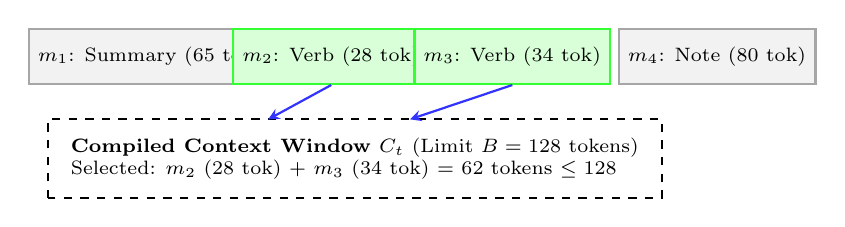
\begin{tikzpicture}[
    item/.style={rectangle, draw=gray!70, fill=gray!10, thick, minimum height=0.7cm, align=center, font=\scriptsize},
    active/.style={rectangle, draw=green!80, fill=green!15, thick, minimum height=0.7cm, align=center, font=\scriptsize},
    flow/.style={->, >=stealth, thick, color=blue!80}]

\node[item, minimum width=2.2cm] (m1) {$m_1$: Summary (65 tok)};
\node[active, minimum width=1.5cm, right of=m1, xshift=1.3cm] (m2) {$m_2$: Verb (28 tok)};
\node[active, minimum width=1.8cm, right of=m2, xshift=1.3cm] (m3) {$m_3$: Verb (34 tok)};
\node[item, minimum width=2.5cm, right of=m3, xshift=1.6cm] (m4) {$m_4$: Note (80 tok)};

\draw[draw=black, dashed, thick] (-1.3, -1.8) rectangle (6.5, -0.8);
\node[font=\scriptsize, align=left] at (2.6, -1.3) {\textbf{Compiled Context Window $C_t$} (Limit $B=128$ tokens)\\Selected: $m_2$ (28 tok) + $m_3$ (34 tok) = 62 tokens $\le 128$};

\draw[flow] (m2.south) -- (1.5, -0.8);
\draw[flow] (m3.south) -- (3.3, -0.8);

\end{tikzpicture}%
}
